
\section{Results}

The model was tested in several scenarios. First, the price 
dynamics and order book evolution are studied with a simple one market settings in which the dividend
yield and interest rate are set to zero. Then the same aspects are investigated
using more complex settings: only some of the traders are allowed to place orders
per trading session and the dividend yield and interest rate are set to random walk.
Then arbitrage is studied using 
a setting in which there exists two identical markets.


\subsection{Single asset simulation}
% Price dynamics, stylized facts, order book evolution
The single asset simulation was run three times: first run
was conducted with a starting market price of 500, second
with a starting market price of 1 500 and third with a starting
price of 1 000 which is near the equilibrium price. The rationale
for this equilibrium price is discussed later.
The first and second simulations were
used to study how the convergence to the equilibrium price occurs
and the third to examine the stylized facts of the price
dynamics after the equilibrium is reached. The simulations were
run using 10 000 zero intelligent traders which is the 
same amount of traders than what \citet{Raberto05} used in their experiments
with moderately similar settings. As only the converge to equilibrium is 
point of interest in the first and second simulations, the number of sessions
were chosen relatively small, 200 sessions, but to get reliable results for
the third simulation the number of sessions were chosen to be 4 000.

The amount of currency and the amount of stock 
a trader owns in the beginning of all of the simulations were set to
10 000 000 units and 10 000 units respectively. Therefore
the ratio of stock to currency is 1 000 which
is the expected equilibrium price as there are
no payouts in either asset. The amount of currency
per trader may seem much but as the tick size is one,
it may be more convenient to think the currency in amounts
in cents or pennies. The standard deviation of
the normal distribution that the traders use to pick the order prices
is set to 20.

%\begin{table}
%    \input{tables/simulation_summary.tex}% table.tex > \mytable
%\end{table}


\subsubsection{Converge to Equilibrium}
% Descriptive analysis
The evolution of trade prices, quantities and values thorough
the trading sessions for the lower and higher starting price simulations 
are shown in the figure ~\ref{fig:basic_trades}. As can be observed,
the near equilibrium market price is achieved in around 30 trading
sessions for both runs. The simulation with lower starting price converges
to the equilibrium in almost instantly whereas for the higher starting
price it takes more sessions. Furthermore, the traded quantities are
initially lower for the simulation with higher staring price than 
for the simulation with lower price. As the traded volumes are lower,
the converge occurs slower due to that there are less situations in
which the market price can adapt. In addition to these findings, 
the equilibrium price is a slightly lower than the expected which is 
about 940.
%The reason why the price stays slightly 
%under the equilibrium price and why the price converges quicker with
%lower starting price than with the higher may be caused by the implementation of
%determining the order price and order quantity. If a trader decides
%to allocate less currency on an order than the order price it chose 
%the order gets obviously invalidated but there is no such
%limitation for placing asks. Therefore there might be a slightly less
%bids than asks in general.

\begin{figure}
    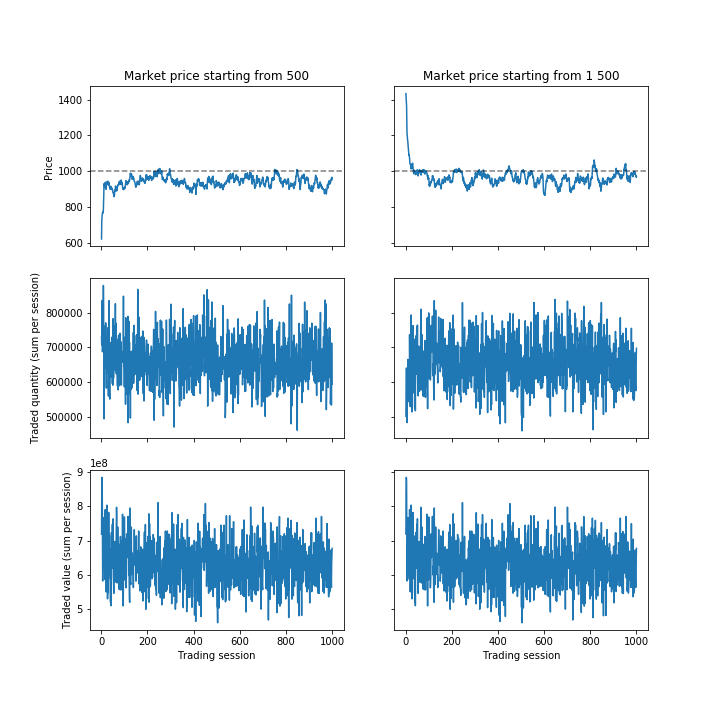
\includegraphics[width=\linewidth]{plots/basic_trades.png}
    \caption{Evolution of price and quantity}
    \label{fig:basic_trades}
\end{figure}

% How the market converged to equilibrium
The market depths shown in figure ~\ref{fig:market_depths} suggests that the
converge to equilibrium is caused by balancing the sides of the market. 
In this figure, the order book is visualized for the first 15 trading sessions. 
The surface describes the evolution of the cumulative bids and cumulative asks 
throughout time and the bottom of the formed valley in the surface is the bid-ask spread. 
The left side from the valley is the the bid book and the right is the ask book. The 
ask side of the market is almost completely missing initially in the run that
starts with lower market price while the opposite is true for the run with higher
initial market price. The ask side of the order book emerges almost instantly 
in the simulation of the lower starting price whereas the converge happens more 
gradually with higher starting price.


\begin{figure}
    \centering
    \begin{subfigure}{.5\textwidth}
      \centering
      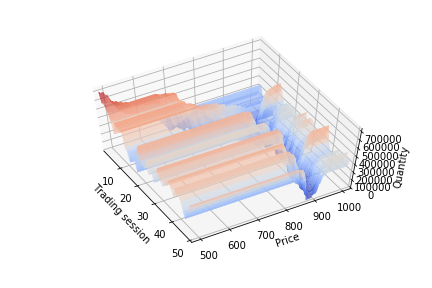
\includegraphics[width=\linewidth]{plots/basic_market_depth_converge_lower.png}
      \caption{Starting price 500}
      \label{fig:market_depth_lower}
    \end{subfigure}%
    \begin{subfigure}{.5\textwidth}
      \centering
      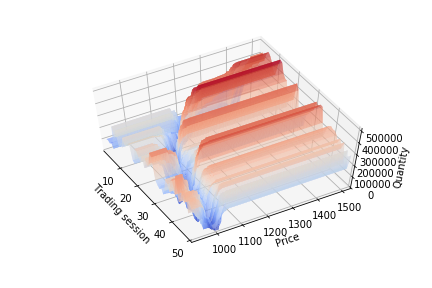
\includegraphics[width=\linewidth]{plots/basic_market_depth_converge_higher.png}
      \caption{Starting price 1 500}
      \label{fig:market_depth_higher}
    \end{subfigure}
    \caption{Converge of the order book to equilibrium}
    \label{fig:market_depths}
\end{figure}

Figure ~\ref{fig:basic_orderbook_evo} provide more top-down view of the orderbook.
This figure shows mostly the same aspects as ~\ref{fig:market_depths} but the sides of the 
order book are not expanded to the edges of the plot and white color represent absence of orders.
The figure suggests that the asking traders in the lower initial market price scenario
adopt the equilibrium price quicker than the bidding traders in higher initial market 
price scenario. One possible cause for this phenomenon might be the buyer-seller asymmetricity
discussed earlier. For example, the downward spikes found in the figure when the equilibrium
is reached is most likely caused by that some traders had consumed their currency balances and decided 
still to do a bid order. Because of the budget constrain, the traders had submitted bid orders with prices
they could afford which were significantly lower than the market price.

\begin{figure}
    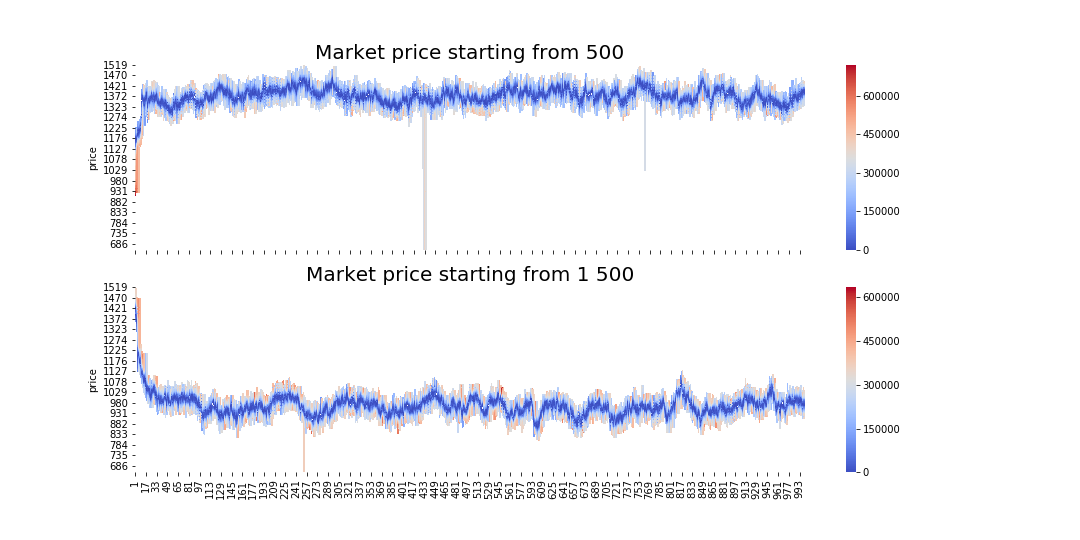
\includegraphics[width=\linewidth]{plots/basic_order_book_evo.png}
    \caption{Order book evolution}
    \label{fig:basic_orderbook_evo}
\end{figure}

When the equilibrium is reached, the order book is rather steep as is illustrated in the figure
~\ref{fig:basic_orderbook_evo}. This figure consists of the last 50 sessions of the extended simulation.
The spread also is also stable most likely due to the number of traders. 

\begin{figure}
    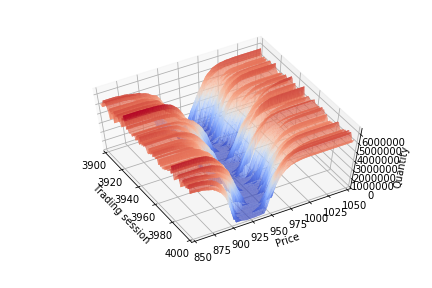
\includegraphics[width=\linewidth]{plots/basic_market_depth_in_equilibrium.png}
    \caption{Order book depth in equilibrium}
    \label{fig:basic_orderbook_evo}
\end{figure}


\subsubsection{Stylized Facts}
% stylized facts
% Somethging about filtering fist 100 out and now inspecting stylized facts
As stated before, the representativeness of real markets is inspected using
stylized facts. In order to have represenative data set to test the facts, the
sessions before reaching the price equilibrium are filtered out. 
As already discussed, the simulation that starts near equilibrium price
is used to study the presence of stylized facts in the model. 

% Autocorrelation
% TODO: REWRITE
The autocorrelation function (ACF) and partial autocorrelation function (PACF) for the prices between
trades are plotted in the figure ~\ref{fig:basic_autocorr}. There is some negative autoregressive
(AR) process in the absolute returns as the ACF plot shows negative and slowly decaying lags 
the line of significance. There are numerous significant lags in the AR process as can be observed from 
the PACF plot. In addition, the prices themselves are positively autocorrelated with an AR process.
These findings are inline with the experiments conducted by \citet{Raberto05}: they also observed
some negative autocorrelation in intraday returns and long lasting autocorrelation in the absolute
values with their simulation. However, it should be noted that this figure shows very short term
autocorrelation and the time between the lags may not be fixed: one lag is simply derived from one
trade. 
% https://www.youtube.com/watch?v=R-oWTWdS1Jg


\begin{figure}
    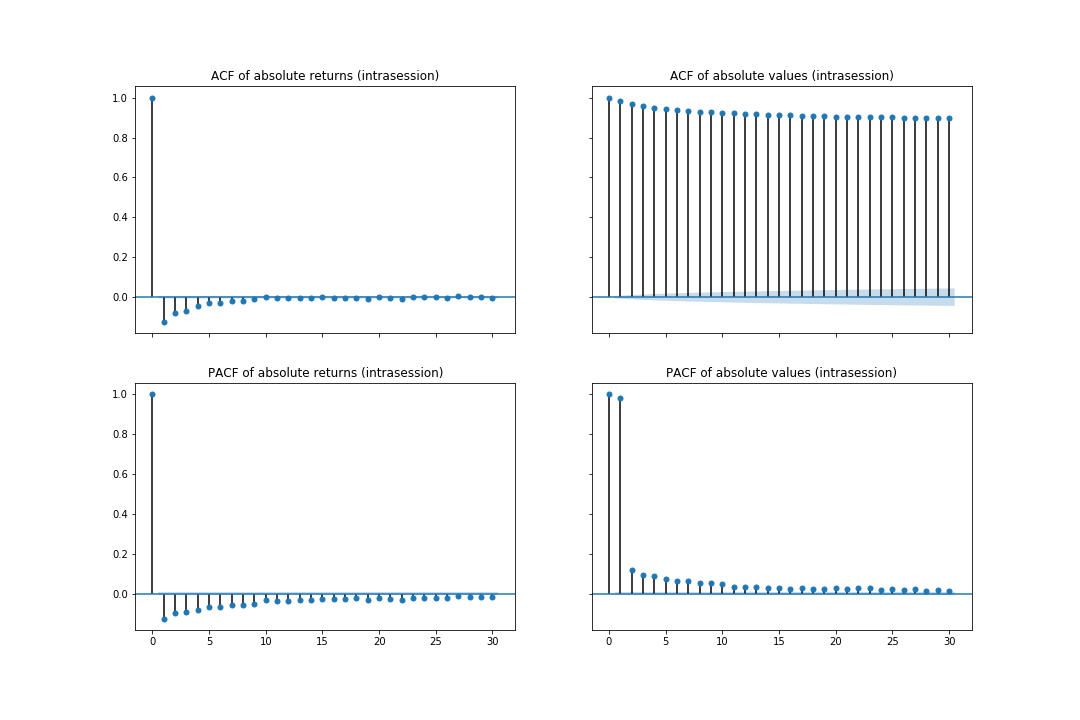
\includegraphics[width=\linewidth]{plots/basic_autocorrelation_intra.png}
    \caption{Autocorrelation of the simulation}
    \label{fig:basic_autocorr}
\end{figure}

Figure ~\ref{fig:basic_autocorr_per_session} suggests that the the autocorrelation is carried over one
session for the absolute returns and four sessions in terms of prices. One lag in the first column of the 
figure is the absolute return between the end of sessions and in the second column the last price per session. 
As can be interpret from the figure, there is an AR(1) process in the absolute returns per session and AR(4) 
for prices on session basis.

\begin{figure}
    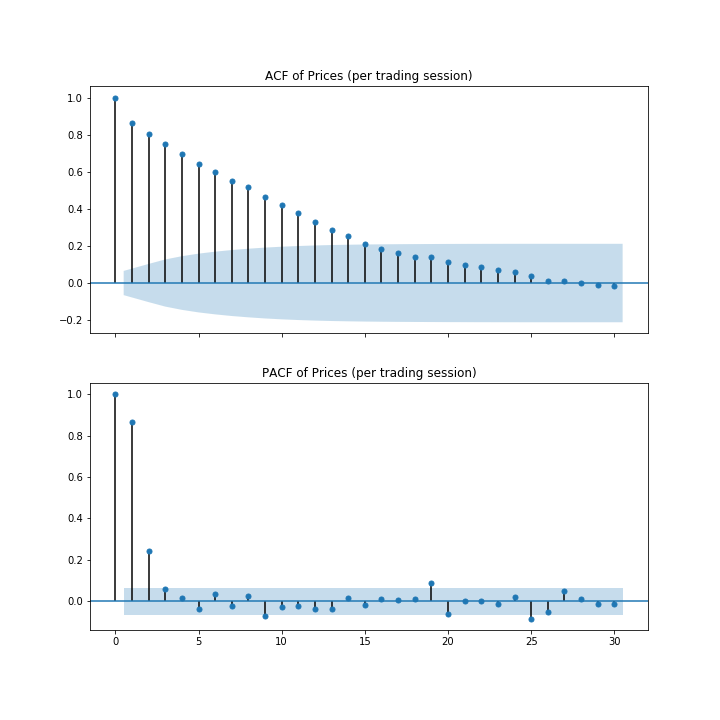
\includegraphics[width=\linewidth]{plots/basic_autocorrelation.png}
    \caption{Autocorrelation of the simulation grouped by session}
    \label{fig:basic_autocorr_per_session}
\end{figure}



% Fat-tailed returns
The distribution of the returns are plotted in ~\ref{fig:basic_return_distr}. As observed in the plot, the fat-tailed returns
clearly exists in the intrasession period but not necessarily per session basis. For intrasession returns, there is a clear spike in the mean of the 
distribution and the tails spread out but these are not visible in the returns between session. In addition, the per session distribution
is not smooth even though the sample consists of 22 million trades. The cause for this may be that the prices are not 
continuous because of the tick size: the minimum possible amount for the price to go up or down is one. Furthermore, prices are
stationary thus the returns are produced by a set of prices. Therefore the returns are also discrete. One option
to mitigate this would be to increase the the amount of currency in order to increase the price and increase the typical
variation of the prices. Jarque-Bera goodness of fit test suggests that both of the time periods are not normally distributed,
as the p-values are practically zero in both cases thus the zero hypothesis is rejected which is a joint hypothesis that the
distribution has no skewness and excess kurtosis. However, as discussed the distributions are not convincingly continuous thus
it is unclear how robust these results are. The kurtosis of the distributions are 5.0 for intrasession and -0.5 for session basis
and therefore this indicates that the intrasession returns are leptokurtic while the returns between sessions the distribution is
. In other words do have fatter tails than normal distribution, 
but is not the case for per session.


% \citet{Raberto05} found fat tails in intra day


\begin{figure}
    \centering
    \begin{subfigure}{.5\textwidth}
        \centering
        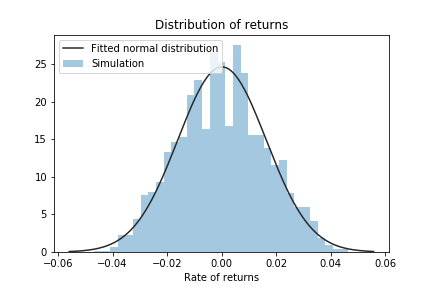
\includegraphics[width=\linewidth]{plots/basic_fat_tails_per_session.png}
        \caption{Between last prices of sessions}
        \label{fig:basic_return_distr_per_session}
    \end{subfigure}%
    \begin{subfigure}{.5\textwidth}
        \centering
        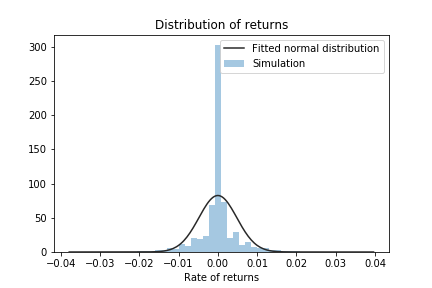
\includegraphics[width=\linewidth]{plots/basic_fat_tails_intrasession.png}
        \caption{Between trades}
        \label{fig:basic_return_distr_intrasession}
    \end{subfigure}
    \caption{Distributions of rate of returns}
    \label{fig:basic_return_distr}
\end{figure}

The spike in the distribution of the intrasession returns may be caused by the structure of the order book. If the order book 
sides are steep, as they are and illustrated in ~\ref{fig:basic_orderbook_evo}, it requires substantially sized 
order to push the opposing side back and have a significant effect on the price. Therefore the price changes between trades 
are generally rather small until there comes an order that can buy or sell significant chunk of the opposing side and have 
instant impact on the price. In such a case the opposing side may be weakened so much that the price change can be radical. 
Therefore the reason for the spike in the returns may be that small and medium sized orders may have similar impact on the 
price but big orders may push the side relatively much more further as the density of the order quantitity drops when moving 
further away from the last market price.

% Volatility clusters
The autocorrelation of the volatilities in figure ~\ref{fig:basic_volaclusters}
indicate there are some volatility clusters in short term. The figure was conducted by
dividing the trade prices to a fixed length windows in which the volatilities were calculated per
window basis. As ACF plot is slowly decaying, the autocorrelation follows AR process. The market 
microstructure is able to produce volatility clusters without additional volatility feedback mechanics.
Furthermore, the order book evolution may play a role in the creating the volatility clusters.

\begin{figure}
    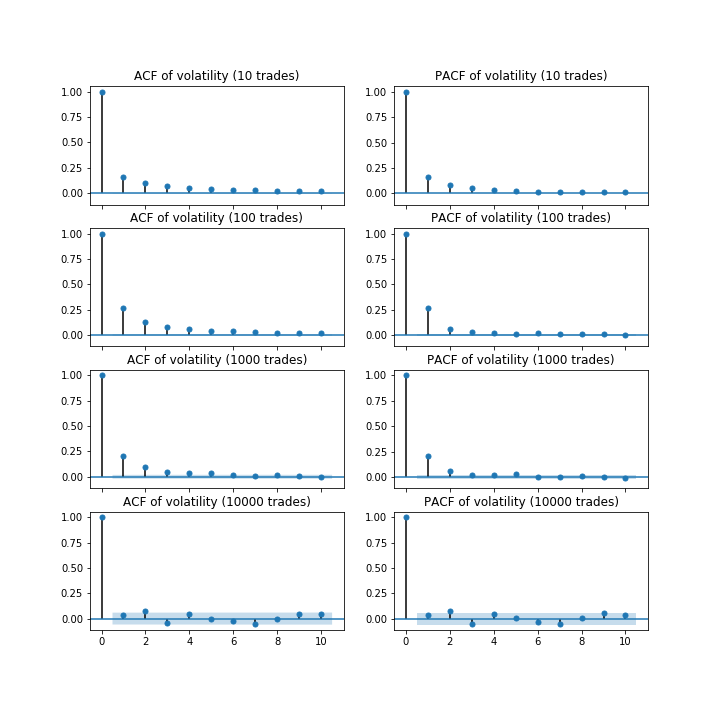
\includegraphics[width=\linewidth]{plots/basic_volaclusters_intra.png}
    \caption{Volatility Clusters}
    \label{fig:basic_volaclusters}
\end{figure}

These findings are somewhat inline with previous literature. \citet{Genoa01}, \citet{Raberto05} and \citet{LIU20082535} 
discussed that the microstructure is the cause for the fat tailed returns. This is probably also the cause for the
fat tails observed in this thesis. However, the autocorrelation is different than what \citet{LIU20082535} observed
with high call market clearing frequencies. Regardless, the autocorrelations of returns observed in this thesis and in their model
are both short term. Even thought a call market has different mechanics than a continuous market, a call market with
very high clearing frequency behaves similar than a continuous market. \citet{Genoa01} and \citet{Raberto05} only discussed
about forming volatility clusters in the context of their model which had volatility feedback mechanism thus it is unclear
whether the volatility clusters observed in the model created in this thesis are to be expected.

\subsection{Arbitrage simulation}

To contribute to \citet{Mil08}'s work to expand situations in which a market populated with zero-intelligent
traders do not produce efficient results, the second experiment is about to study the arbitrage in 
zero-intelligent markets. The 
conducted with similar settings as the
first experiment but instead of one market there are two indentical markets. The se
